\documentclass[12pt,a4paper]{article}
\usepackage[left=1cm,right=1cm,top=1.5cm,bottom=1.5cm,a4paper]{geometry}

\usepackage{amsmath}
\usepackage{amsfonts}
\usepackage{amssymb}
\usepackage{makeidx}
\usepackage{graphicx}
\usepackage{amsthm}
\usepackage{mathtools} 

\usepackage{commath} %absolute value
\usepackage{siunitx} %degree

\usepackage{hyperref}

\usepackage{color}
\usepackage{tcolorbox}
\usepackage{enumerate}
\usepackage{booktabs}
\usepackage{dashrule}
\usepackage{multirow}

\newcommand{\dispsty}{\displaystyle}

\newcommand{\makeline}{\rule{\linewidth}{1pt}}
\newcommand{\makedashline}{\hdashrule[0.5ex]{\linewidth}{0.5pt}{2mm}}
\newcommand{\sol}{\textcolor{magenta}{\bf \textit{Sol.}}\quad}
\newcommand{\eg}{\textcolor{blue}{\bf e.g.)\ }}
\newcommand{\ie}{\textit{i.e.}}
\newcommand{\remark}{\textcolor{cyan}{\textbf{\textit{Remark.}\ }}}

\newcommand{\Var}{\text{Var}}
\newcommand{\sd}{\text{sd}}
\newcommand{\mean}[1]{\bar{#1}}
\newcommand{\Cov}{\textit{Cov}}
\newcommand{\Corr}{\textit{Corr}}
\newcommand{\SE}{\text{S.E.}}
\newcommand{\df}{\text{d.f.}}

\author{Hacker-Code.J}
\title{\bf\Huge Mathematical Statistics}

\begin{document}
\maketitle
\tableofcontents
\newpage

\begin{tcolorbox}[colback=white]
	
\end{tcolorbox}

\section{Introduction}

\section{Organization and Description of Data}

\subsection{Main Types of Data}
%\begin{enumerate}
%	\item \textbf{Qualitative} or \textbf{categorical} data
%	\item \textbf{Numerical} or \textbf{measurement} data \\
%	\\
%	We will use the term \textbf{numerical-valued variable}(or just \textbf{variable}) to refer to a characteristic that is measured on a numerical scale. \begin{itemize}
%		\item[-] \textbf{discrete value}: \textit{countable} \par
%		The name \textbf{discrete} draws from the fact that the scale is made up of distinct numbers with gaps in between.
%		\item[-] \textbf{continuous variable}: \textit{uncountable}
%	\end{itemize}
%\end{enumerate}
%
\subsection{Describing Data by Tables and Graphs}
%
\subsection{Measures of Center}
%The most important aspect of studying the distribution of a sample of measurements is locating the position of a central value about which the measurements are distributed. Two most commonly used indicators of center are the \textbf{mean} and the \textbf{median}. \par
%The \textbf{mean}(or \textbf{average}) of a set of measurements is the sum of the measurements divided by their number. \begin{tcolorbox}
%	The \textbf{sample mean} of a set of $n$ measurements $x_1, x_2.\cdots. x_n$ is the sum of the measurements divided by $n$. The sample mean is denoted by $\bar{x}$ \[
%	\bar{x}=\frac{1}{n}(x_1+x_2+\cdots+x_n)=\frac{1}{n}\sum_{i=1}^nx_i
%	\]
%\end{tcolorbox} 
%The \textbf{sample median} of a set of $n$ measurements $x_1, \cdots, x_n$ is the middle value when the measurements are arranged from smallest to largest.
%
\subsection{Measures of Variation}
Besides locating the center of the data, any descriptive study of data must numerically measure the extent of variation around the center. 
\subsubsection{Deviation}
\begin{align*}
	\text{Deviation} &= \text{Observation} - (\text{Sample mean}) \\
	&= x - \mean{x}.
\end{align*}
For any data set, the total deviation is 0, that is, \[
\sum\text{Deviations} = \sum(x-\mean{x})=0.
\] \textbf{Check.} Since $\mean{x}=\frac{\sum_{i=1}^nx_i}{n}$, \ie, $\sum_{i=1}^nx_i=x_1+x_2+\cdots+x_n=n\mean{x}$, \begin{align*}
	\sum_{i=1}^n(x_i-\mean{x}) &= (x_1-\mean{x}) + (x_2-\mean{x}) + \cdots + (x_n-\mean{x}) \\
	&= x_1+x_2+\cdots+x_n-n\mean{x} \\
	&= n\mean{x} - n\mean{x} = 0.
\end{align*}

\subsubsection{Sample Variance and Sample Standard Deviation}
\begin{tcolorbox}[colback=white]
	\textbf{Sample Variance} of $n$ observations: \[
		s^2=\frac{\text{Sum of squared deviations}}{n-1} = \frac{\sum_{i=1}^n(x_i-\mean{x})^2}{n-1}
	\]
\end{tcolorbox}\
\remark Although the sample variance is conceptualized as the \textbf{average squared deviation}, notice that the divisor is $n-1$ rather than $n$. The divisor, $n-1$, is called the degrees of \textit{freedom}\footnote[1]{
The deviations add to 0 so a specification of any $n-1$ deviations allows us to recover the one that is left out. In definition of $s^2$, the divisor $n-1$ represents the number of deviations that can be viewed as free quantities.} associated with $s^2$.\\
\begin{tcolorbox}[colback=white]
	\begin{center}
		\textbf{Sample Standard Deviation}
	\end{center} \[
	s=\sqrt{\text{Variance}} = \sqrt{\frac{\sum_{i=1}^n(x_i-\mean{x})^2}{n-1}}
	\]
\end{tcolorbox}\
\\
\begin{tcolorbox}[colback=white]
	An alternative formula for the sample variance is \[
	s^2=\frac{1}{n-1}\left[\sum x_i^2-\frac{(\sum x_i)^2}{n} \right]
	\] \begin{proof}
		Note that \begin{align*}
		\sum(x_i-\mean{x})^2&=\sum x_i^2 - \sum2x_i\mean{x} +\sum\mean{x}^2 \\
		&=\sum x_i^2 - 2\mean{x}\sum x_i +n\mean{x}^2.
		\end{align*} Then, since $\mean{x}=\sum x_i/n$, \begin{align*}
		\sum(x_i-\mean{x})^2 &= \sum x_i^2 - 2\frac{\sum x_i}{n}\sum x_i +n\left(\frac{\sum x_i}{n}\right)^2 \\
		&= \sum x_i^2 - 2\frac{(\sum x_i)^2}{n} +\frac{(\sum x_i)^2}{n} \\
		&= \sum x_i^2 - \frac{(\sum x_i)^2}{n}.
		\end{align*}
	\end{proof}	
\end{tcolorbox}\
\\
It does not require the calculation of the individual deviations.

\subsubsection{Population Mean and Sample Mean}
\ \begin{center}
	\begin{tabular}{c||c|c}
	\toprule[1.2pt]
	& \textbf{Population}($N$) & \textbf{Sample}($n$) \\
	\hline
	&&\\
	Mean & \(\dispsty\mu = \frac{\sum_{i=1}^Nx_i}{N} \) & \(\dispsty\mean{x} = \frac{\sum_{i=1}^nx_i}{n-1} \)\\&&\\
	\hline&&\\
	Variance & \(\dispsty \sigma^2 = \frac{\sum(x-\mu)^2 }{N} \) & \(\dispsty s^2 = \frac{\sum(x-\mean{x})^2 }{n-1} \)\\&&\\
	\bottomrule[1.2pt]
\end{tabular}
\end{center}\begin{tcolorbox}[colback=white]\[
	\frac{1}{n}\sum_{i=1}^n(x_i-\mean{x})^2=\frac{1}{n}\sum_{i=1}^n(x_i-\mu)^2-(\mean{x}-\mu)^2
	\] \begin{proof}\begin{align*}
		\frac{1}{n}\sum_{i=1}^n(x_i-\mu)^2&=\frac{1}{n}\sum_{i=1}^n(x_i-\mean{x}+\mean{x}-\mu)^2 \\
		&=\frac{1}{n}\sum_{i=1}^n\left[(x_i-\mean{x})^2+2(x-\mean{x})(x-\mu)+(\mean{x}-\mu)^2\right] \\
		&=\frac{1}{n}\left[\sum_{i=1}^n(x_i-\mean{x})^2+2(x-\mu)\underset{\textcolor{red}{=0}}{\underline{\sum_{i=1}^n(x-\mean{x})}}+\sum_{i=1}^n(\mean{x}-\mu)^2 \right] \\
		&= \frac{1}{n}\sum_{i=1}^n(x_i-\mean{x})^2+(\mean{x}-\mu)^2
	\end{align*}
	\end{proof}
\end{tcolorbox}

\subsubsection{Other Measure of Variation}
\begin{tcolorbox}[colback=white]
	\centering
	\textbf{Sample range} = Largest observation - Smallest observation
\end{tcolorbox}\
The range gives the length of the interval spanned by the observations.


\section{Descriptive Study of Bivariate Data}

\subsection{Simpson's Paradox}

\subsection{Scatter Diagram of Bivariate Measurement Data}

\subsection{The Correlation Coefficient - A Measure of Linear Relation}
Our visual impression of the closeness of the scatter to a linear relation can be quantified by calculating a numerical measure, called the \textbf{correlation coefficient} and denoted ``$r$''.\\
\\
Important features of correlation coefficient:

\subsubsection{Calculation of $\boldsymbol{r}$}
The sample correlation is calculated from $n$ pairs of observations on the two characteristics \[
(x_1, y_1), (x_2, y_2), \cdots, (x_n, y_n).
\] The correlation coefficient is best interpreted in terms of the \textbf{standardized observation}, or \textbf{sample $\boldsymbol{z}$ values} \[
\frac{\text{Observation}-\text{Sample mean}}{\text{Sample standard deviation}} = \frac{x_i-\bar{x}}{s_x}
\] where $s_x=\sqrt{\sum_{i=1}^n(x_i-\bar{x})^2/(n-1)}$ and the subscript $x$ on $s$ distinguishes the sample the sample standard deviation of the $x$ observation from the sample standard deviation $s_y$ of the $y$ observations.\par
The \textbf{sample correlation coefficient} is the sum of the products of the standardized $x$ observation times the standardized $y$ observation divided by $n-1$.
\begin{tcolorbox}[colback=white]\begin{center}
		\textbf{Sample Correlation Coefficient}
	\end{center} \[
	r=\frac{1}{n-1}\sum_{i=1}^n\left(\frac{x_i-\bar{x}}{s_x}\right)\left(\frac{y_i-\bar{y}}{s_y}\right)
\]	
\end{tcolorbox}

\begin{tcolorbox}[colback=white]\begin{center}
		\textbf{Calculation Formula for the Sample Correlation Coefficient}
	\end{center} \[
	r= \frac{S_{xy}}{\sqrt{S_{xx}}\sqrt{S_{yy}}}
	\] where \begin{align*}
		S_{xy} &= \sum(x-\mean{x})(y-\mean{y}) \\
		S_{xx} &= \sum(x-\mean{x})^2,\quad S_{yy}= \sum(y-\mean{y})^2
	\end{align*}
\end{tcolorbox}

\begin{tcolorbox}[colback=white]\[
		S_{xx} = \sum x^2 - \frac{(\sum x)^2}{n},\ S_{yy} = \sum y^2 - \frac{(\sum y)^2}{n},\ \text{and}\ S_{xy} = \sum xy - \frac{(\sum x)(\sum y)}{n}.
		\]\begin{proof} Since $(x-\mean{x})(y-\mean{y})=xy-x\mean{y}-\mean{x}y+\mean{x}\mean{y}$, \[
		\sum(x-\mean{x})(y-\mean{y})=\sum xy-\mean{y}\sum x-\mean{x}\sum y+n\mean{x}\mean{y}.
		\] Then, since $\mean{x}=\sum x/n$ and $\mean{y}=\sum y/n$, \begin{align*}
		\sum(x-\mean{x})(y-\mean{y})&=\sum xy-\frac{\sum y}{n}\sum x-\frac{\sum x}{n}\sum y+n\frac{\sum x}{n}\frac{\sum y}{n} \\
		&= \sum xy - \frac{2\sum x\sum y}{n} + \frac{\sum xy}{n} \\
		&=\sum xy - \frac{\sum x\sum y}{n}
		\end{align*}
	\end{proof}
\end{tcolorbox}\
\\
\eg\textcolor{blue}{\bf Calculation of Sample Correlation}\quad Calculate $r$ for the $n=4$ pairs of observations \[
(2,5)\quad(1,3)\quad(5,6)\quad(0,2) 
\] \begin{proof}[\sol]\
	\begin{center}
		\begin{tabular}{cccccccc||ccc}
		\toprule[1.2pt]
		& $x$ & $y$ & $x-\mean{x}$ & $y-\mean{y}$ & $(x-\mean{x})^2$ & $(y-\mean{y})^2$ & $(x-\mean{x})(y-\mean{y})$ & $x^2$ & $y^2$ & $xy$\\
		\hline
		& 2& 5& 0& 1& 0& 1& 0 & 4& 25& 10\\
		& 1& 3& -1& -1& 1& 1& 1 & 1& 9& 3\\
		& 5& 6& 3& 2& 9& 4& 6 & 25& 36& 30\\
		& 0& 2& -2& -2& 4& 4& 4 & 0& 4& 0\\
		\hline
		Total & 8& 16& 0& 0& 14& 10& 11 & 30& 74& 43\\
		& $\mean{x}=2$ & $\mean{y}=4$ & & & $S_{xx}$& $S_{yy}$& $S_{xy}$ & $\sum x^2$ & $\sum y^2$ & $\sum xy$\\
		\bottomrule[1.2pt]
	\end{tabular}
	\end{center} Consequently, \[
	r=\frac{S_{xy}}{\sqrt{S_{xx}}\sqrt{S_{yy}}}=\frac{11}{\sqrt{14}\sqrt{10}}\ =\ .930
\] The value .930 is large and it implies a strong associate where both $x$ and $y$ tend to be small or both tend to be large.
\end{proof}

\subsubsection{Population Correlation Coefficient($\boldsymbol{\rho}$) and Sample Correlation Coefficient($\boldsymbol{r}$)}

\begin{tcolorbox}[colback=white]
	\[
	\rho = \frac{1}{N}\sum_{i=1}^N\left(\frac{c_{1i}-\mu_1}{\sigma_1}\right)\left(\frac{c_{2i}-\mu_2}{\sigma_2}\right)
	\]
\end{tcolorbox}

\begin{tcolorbox}[colback=white]
	\begin{itemize}
		\item $-1\leq\rho\leq 1$
	\end{itemize}\tcblower\begin{proof}\begin{align*}
	0 &\leq \frac{1}{N}\sum_{i=1}^N\left(\frac{c_{1i}-\mu_1}{\sigma_1}-\rho\frac{c_{2i}-\mu_2}{\sigma_2}\right)^2\\
	&= \frac{1}{\sigma_1^2}\cdot\frac{1}{N}\sum_{i=1}^N(c_{1i}-\mu_1)^2-2\rho\cdot\frac{1}{N}\sum_{i=1}^N\left(\frac{c_{1i}-\mu_1}{\sigma_1}\right)\left(\frac{c_{2i}-\mu_2}{\sigma_2}\right)+\frac{\rho^2}{\sigma_2^2}\cdot\frac{1}{N}\sum_{i=1}^N(c_{2i}-\mu_2)^2 \\
	&=1-2\rho^2+\rho^2 \\
	&=1-\rho^2.
	\end{align*} Thus, $\rho^2\leq1$, i.e, $-1\leq\rho\leq 1$.
\end{proof}
\end{tcolorbox}

\subsubsection{Correlation and Caution}
\begin{tcolorbox}[colback=white]
	An observed correlation between two variables may be \textbf{spurious}. That is, it may be caused by the influence of a third variable.
\end{tcolorbox}


\section{Probability}

\subsection{Probability of an Event}

\begin{tcolorbox}[colback=white]
	An \textbf{experiment} is the process of observing a phenomenon that has variation in its outcomes.
\end{tcolorbox}

\begin{tcolorbox}[colback=white]
	\begin{itemize}
	\item The \textbf{sample space} $S$ associated with an experiment is \underline{the collection} of all
	possible distinct outcomes of the experiment. \begin{itemize} \item Each outcome is called an elementary outcome, a simple event, or an element of the sample space, say, $e_1, e_2, \cdots$. \end{itemize}
	\item An \textbf{event} $A, B$ is the set of elementary outcomes possessing a designated feature. ($A,B\subseteq S$) \begin{itemize}
		\item An event $A$ occurs when any one of the elementary outcomes in $A$ occurs.
	\end{itemize}
	\end{itemize}
\end{tcolorbox}\
\begin{tcolorbox}[colback=white]
	The \textbf{probability of an event} is a numerical value that represents the proportion of times the event is expected to occur when the experiment is repeated many times under identical conditions. (Relative Frequency) \\
	\\
	The probability of event A is denoted by P(A).\\ \begin{tcolorbox}[colback=white]
		\textbf{Probability} must be satisfy: \begin{enumerate}
			\item \(0\leq P(A)\leq1 \) for all events $A$
			\item \(\dispsty P(A)=\sum_{\text{all}\ e\in A}P(e) \)
			\item \(\dispsty P(S)=\sum_{\text{all}\ e\in S}P(e) =1 \)
		\end{enumerate}
	\end{tcolorbox}
\end{tcolorbox}

\subsection{Methods of Assigning Probability}

\subsubsection{Equally Likely Elementary Outcomes\_ The Uniform Probability Model}
\eg Consider the experiment of rolling a fair die and recording top face. Then \[
S=\{e_1, e_2, \cdots, e_6\}
\] \[
P(e_1)=P(e_2)=\cdots=P(e_6)=\frac{1}{6}
\]
\textbf{Q.} What is the probability of getting a number higher than $4$? \\
\textbf{A.} Note that $A=\{e_5,e_6\}$. \[
P(A)=P(e_5)+P(e_6)=\frac{1}{6}+\frac{1}{6}=\frac{1}{3}.
\]

\subsubsection{Probability as The Long-Run Relative Frequency}
Letting $N$ denote the number of repetition (or trials) of an experiment, we set \begin{align*}
		\text{Relative frequency of event}\ A\ \text{in}\ N\ \text{trials} &= \frac{\text{No. of times}\ A\ \text{occurs in}\ N\ \text{trials}}{N} \\ &= P_N. 
\end{align*}Then \[
	P(A) = \lim\limits_{N\to\infty}P_N.
\] We define $P(A)$, the probability of an event $A$, as the value to which the
relative frequency stabilizes with increasing number of trials. \par
Although we will never know $P(A)$ exactly, it can be estimated accurately by repeating the experiment many times.

\subsection{Event Relation and Two Laws of Probability}
For event $A$, \begin{itemize}
	\item complement: $A^C$, $\bar{A}$
	\item union: $A\cup B$
	\item intersection: $A\cap B$, $AB$
\end{itemize}
Two events $A$, $B$ are mutually disjoint $\iff A\cap B=\varnothing$, \ie, $AB=\varnothing$  
\\
\begin{tcolorbox}[colback=white]
	(\textbf{Law of Complement}) $P(A)=1-P(\bar{A})$
\end{tcolorbox}
\begin{tcolorbox}[colback=white]
	(\textbf{Addition Law}) $P(A\cup B)=P(A)+P(B)-P(AB)$
\end{tcolorbox}

\subsection*{4.*\ \ \ Axioms of Probability}
\addcontentsline{toc}{subsection}{4.*\ \ \ Axioms of Probability}
If $P(A)$ satisfies as follows: \begin{enumerate}
	\item For any event $A$, $0\leq P(A)\leq 1$.
	\item $P(S)=1$, where $S$ is sample space.
	\item For events that are mutually disjoint, $A_1,A_2,\cdots$, \[
	P(A_1\cup A_2\cup\cdots)=P(A_1)+P(A_2)+\cdots.
	\] 
\end{enumerate}

\subsection{Conditional Probability and Independence}
The probability of $A$ when it is known that B has occurred is called the conditional probability of A given B and is denoted by $P(A|B)$.
\begin{tcolorbox}[colback=white]
	The \textbf{conditional probability} of $A$ given $B$ is denoted by $P(A|B)$ and defined by the formula
	\[
	P(A|B) = \frac{P(AB)}{P(B)}
	\] Equivalently, this formula can be written \[
	P(AB) = P(B)P(A| B)
	\] This latter version is called the \textbf{multiplication law of probability}.
\end{tcolorbox}

\begin{tcolorbox}[colback=white]
	Two events $A$ and $B$ are \textbf{independent} if \[
	P(A|B) = P(A)
	\] 	 Equivalent conditions are \[
	P(B|A) = P(B)
	\] or \[
	P(AB) = P(A)P(B)
	\] \makedashline \\ \textbf{Check.} \[
	P(A)=P(A|B)=\frac{P(AB)}{P(B)}\quad\Longrightarrow\quad P(AB)=P(A)P(B)
	\]
\end{tcolorbox}\ \\
\textcolor{red}{\textbf{\textit{Caution.}}} Do not confuse the terms ``incompatible events'' and ``independent events''. We say $A$ and $B$ are incompatible when their intersection $AB$ is empty, so $P(AB)=0$. On the other hand, if $A$ and $B$ are independent, $P(AB)=P(A)P(B)$. Both these properties cannot hold as long as $A$ and $B$ have non-zero probabilities.

\subsection{Bayes' Theorem}
An event $A$ can occur either when an event $B$ occurs or when it does not occur. That is, $A$ can be written as the disjoint union of $AB$ and $A\bar{B}$. Consequently, \[
P(A) = P(AB) + P(A\bar{B}).
\]
\begin{tcolorbox}[colback=white]
	(\textbf{Rule of Total Probability})\quad \(P(A)=P(A|B)P(B) + P(A|\bar{B})P(\bar{B}) \)
	\tcblower
	\textbf{Extend.} For events $A_1, A_2, \cdots, A_n$, where $A_1\cup A_2\cup\cdots\cup A_n=S$ and $A_i\cap A_j=\varnothing$ for $i\neq j$, $P(A_i)>0$, \[
	P(B) = P(B|A_1)P(A_1) + P(B|A_2)P(A_2) + \cdots + P(B|A_n)P(A_n)
	\]
\end{tcolorbox}\ \\
\makedashline
\begin{itemize}
	\item (\textbf{prior probability}) Suppose the two events $A$ and $B$ can occur together and, before observing either, we know the probability \[
	P(B)\ \text{so}\ P(\bar{B})=1-P(B).
	\] When we also know the two conditional probabilities $P(A|B)$ and $P(A|\bar{B})$, the probability of $B$ can be updated when we observe the status of $A$.
	\item (\textbf{posterior probability}) Once we know $A$ has occurred, the updated or \textit{posterior probability} of $B$ is given by the condition probability \(\dispsty P(B|A)=\frac{P(AB)}{P(A)} \).
\end{itemize}

\begin{tcolorbox}[colback=white]
	(\textbf{Bayes' Theorem}) \[
	P(B|A) = \frac{P(A|B)P(B)}{P(A|B)P(B)+P(A|\bar{B})P(\bar{B})}
	\] The posterior probability of $\bar{B}$ is then $P(\bar{B}|A)=1-P(B|A)$
\end{tcolorbox}

\section{Probability Distributions}

\subsection{Random Variables}

\begin{tcolorbox}[colback=white]
	A \textbf{random variable} $X$ associates a numerical value with each outcome of an experiment. \[
	X: S\to\mathbb{R},
	\] where $S$ is a sample space and $\mathbb{R}$ is a real number.
\end{tcolorbox}

\subsection{Probability Distribution of a Discrete Random Variable}

\begin{tcolorbox}[colback=white]
	The \textbf{probability distribution}, or simply the \textbf{distribution}, of a discrete random variable $X$ is a list of the distinct numerical values of $X$ along with their associated probabilities. (Often, a formula can be used in place of a detailed list.)
\end{tcolorbox}\
\\
Consider the distinct values of a random variable $X$. The probability that a particular value $x_i$ occurs will be denoted by $f(x_i)$. If $X$ can take $k$ possible values $x_1,\cdots,x_k$ with the corresponding probabilities $f(x_1), \cdots, f(x_k)$, the probability distribution of $X$ can be displayed in the format of below table. \begin{center}\begin{tabular}{c|c}
		\toprule[1.2pt]
		Value of $x$ & Probability $f(x)$ \\
		\hline
		$x_1$ & $f(x_1)$ \\
		$x_2$ & $f(x_2)$ \\
		\vdots & \vdots \\
		$x_k$ & $f(x_k)$ \\
		\hline
		Total & 1 \\
		\bottomrule[1.2pt]
	\end{tabular}
\end{center}

\begin{tcolorbox}[colback=white]
	The \textbf{probability distribution} of a discrete of a random variable $X$ is described as the function \[
	f(x_i) = P(X=x_i)
	\] which gives the probability for each value and satisfies: \begin{enumerate}
		\item $0\leq f(x_i)\leq 1$ for each value $x_i$ of $X$
		\item \(\dispsty\sum_{i=1}^kf(x_i)=1 \)
	\end{enumerate}
\end{tcolorbox}

\subsection{Expectation(Mean) and Standard Deviation of a Probability Distribution}
The sample mean is calculated as \[
\bar{x}=\frac{\text{Sum of the observations}}{\text{Sample size}}.
\] The another calculation of sample mean illustrates the formula \[
\text{Sample mean}\ \bar{x} = \sum(\text{Value}\ \times\ \text{Relative frequency}).
\] If we imagine a huge number of trials, the relative frequencies will approach the probability. The mean of the (infinite) collection of trials should be calculated as \[
\sum(\text{Value}\times\text{Probability}).
\]
\\
Define the mean of a random variable $X$ or its probability distribution as \[
\sum(\text{Value}\times\text{Probability})\quad\text{or}\quad \sum x_if(x_i).
\] where $x_i$'s denote the distinct values of $X$. The mean of a probability distribution is also called the population mean for the variable $X$. \par
The mean of a random values $X$ is called its \textbf{expected value}. \begin{tcolorbox}[colback=white]
	The \textbf{mean} of $X$ or \textbf{population mean} \begin{align*}
		E[X] &= \mu \\
		&= \sum(\text{Value}\ \times\ \text{Probability})=\sum x_if(x_i)
	\end{align*} Here the sum extends over all the distinct values $x_i$ of $X$.
\end{tcolorbox}
Since the mean $\mu$ is the center of the distribution of $X$, we express variation of $X$ in term of the deviation $X-\mu$. We define the variance of $X$ as the expected value of the squared deviation $(X-\mu)^2$
\begin{tcolorbox}[colback=white]\begin{center}
		\textbf{Variance and Standard Deviation of $\boldsymbol{X}$}
\end{center}\begin{align*}
	\sigma^2 &=\Var[X]=\sum(x_i-\mu)^2f(x_i) \\
	\sigma &=\sd[X]= +\sqrt{\Var[X]}
\end{align*}
\end{tcolorbox}
\begin{tcolorbox}[colback=white]
	\centering
	\textbf{Alternative Formula for Hand calculation} \[
	\sigma^2=\sum x_i^2f(x_i) - \mu^2
	\]
\end{tcolorbox}\ \\
\eg\textcolor{blue}{\bf Calculating a Population Variance and Standard Deviation}\quad Calculate the variance and the standard deviation of the distribution of $X$ that appears in the left two columns of below table.
\begin{center}\begin{tabular}{c|c||cccc||c}
	\toprule[1.2pt]
	$x$ & $f(x)$ & $xf(x)$ & $(x-\mu)$ & $(x-\mu)^2$ & $(x-\mu)^2f(x)$ & $x^2f(x)$\\
	\hline
	0&.1& 0 & -2&4&.4&0\\
	1&.2& .2& -1&1&.2&0.2\\
	2&.4& .8& 0&0&.0&1.6\\
	3&.2& .6& 1&1&.2&1.8\\
	4&.1& .4& 2&4&.4&1.6\\
	\hline
	Total&1.0&2.0 = $\mu$&&&$1.2=\sigma^2$&$5.2=\sum x^2f(x)$\\
\end{tabular}
\end{center}\begin{align*}
\Var(X)&=\sigma^2=1.2\quad& \sigma^2=5.2-(2.0)^2=1.2 \\
\sd(X)&=\sigma=\sqrt{1.2}=1.095\quad& \sigma=\sqrt{1.2}=1.095
\end{align*}

\subsection{Successes and Failures - Bernoulli Trails}

\subsubsection{Bernoulli Trials}
\begin{itemize}
	\item The sample space $S = \set{\ \text{S},\ \text{F}\ }$.
	\item The probability of success $p=$P(S), the probability of failure $q=$P(F).
	\item $0\leq p\leq 1$, $q=1-p$.
\end{itemize}
\begin{tcolorbox}[colback=white]
	\centering
	\textbf{Bernoulli Trials} \begin{enumerate}
		\item Each trial yields one of two outcomes, technically called success (S) and failure (F).
		\item For each trial, the probability of success $P$(S) is the same and is denoted by $p = P$(S). The probability of failure is then $P$(F) $= 1-p$ for each trial and is denoted by $q$, so that $p+q=1$.
		\item Trials are independent. The probability of success in a trial remains unchanged given the outcomes of all the other trials.	
\end{enumerate}
\end{tcolorbox}

\subsubsection{Bernoulli Random Variable}
\begin{itemize}
	\item The random variable, $X$(S) = 1 and $X$(F)=0, in $S=\set{\ \text{S},\ \text{F}\ }$.
	\item \textbf{Bernoulli Distribution}: The probability distribution of Bernoulli random variable.\ \begin{center}
		\begin{tabular}{ccc|ccc|ccc}
		\toprule[1.2pt]
		& $x$ &&& 0 &&& 1 & \\
		\hline
		&$p(x)$ &&& $1-p$ &&& $p$ & \\
		\bottomrule[1.2pt]
	\end{tabular}
	\end{center}
\end{itemize}

\subsection{The Binomial Distribution}

\begin{tcolorbox}[colback=white]
	A \textbf{probability model} is an assumed form of the probability distribution that describes the chance behavior for a random variable $X$. \par
	Probabilities are expressed in terms of relevant population quantities, called the \textbf{parameters}.
\end{tcolorbox}
\begin{tcolorbox}[colback=white]
	\begin{center}	
	\textbf{The Binomial Distribution}\end{center}
	Denote \begin{align*}
		n &= \text{a fixed number of Bernolli trials} \\
		p &= \text{the probability of success in each trial} \\
		X &= \text{the (random) number of successes in $n$ trials}
	\end{align*} The random variable $X$ called a \textbf{binomial random variable}. Its distribution is called a \textbf{binomial distribution}.
\end{tcolorbox}\ \\
\eg\textcolor{blue}{\bf An Example of the Binomial Distribution}\quad The elementary outcomes of 4 samples, the associated probabilities, and the value of $X$ are listed as follows. \begin{center}
	\begin{tabular}{ccc ccc ccc ccc ccc}
	& FFFF &&& SFFF &&& SSFF &&& SSSF &&& SSSS & \\
	& 	   &&& FSFF &&& SFSF &&& SSFS &&& & \\
	& 	   &&& FFSF &&& SFFS &&& SFSS &&& & \\
	& 	   &&& FFFS &&& FSSF &&& FSSS &&& & \\
	& 	   &&&      &&& FSFS &&& &&& & \\
	& 	   &&&      &&& FFSS &&& &&& & \\
\end{tabular}\end{center}
\begin{center}\begin{tabular}{c||ccccc}
	\toprule[1.2pt]
	Value of $X$ & 0 & 1 & 2 & 3 & 4 \\
	\hline
	Probability of each outcome & $q^4$ & $pq^3$ & $p^2q^2$ & $p^3q$ & $p^4$ \\
	\hline
	Number of outcomes & $1=\binom{4}{0}$ & $4=\binom{4}{1}$ & $6=\binom{4}{2}$ & $4=\binom{4}{1}$ & $1=\binom{4}{4}$ \\
	\bottomrule[1.2pt] 
\end{tabular}\end{center}
\begin{center}\begin{tabular}{c||ccccc}
	\toprule[1.2pt]
	Value $x$ & 0 & 1 & 2 & 3 & 4 \\
	\hline
	Probability $f(x)$ & $\binom{4}{0}p^0q^4$ & $\binom{4}{1}p^1q^3$ & $\binom{4}{2}p^2q^2$ & $\binom{4}{1}p^3q^1$ & $\binom{4}{4}p^4q^0$ \\
	\bottomrule[1.2pt]
\end{tabular}
\end{center}

\begin{tcolorbox}[colback=white]
	The \textbf{binomial distribution} with $n$ trails and success probability $p$ is described by the function \[
	f(x) = P[X=x] = \binom{n}{x}p^x(1-p)^{n-x}
	\] for the possible values $x = 0, 1, \cdots, n$.
\end{tcolorbox}

\subsubsection{The Mean and Standard Deviation of the Binomial Distribution}
\[
X=X_1+X_2+\cdots+x_n\sim B(n,p)
\] \begin{itemize}
	\item \(E[X]=E[X_1] + \cdots + E[X_n] = np \)
	\item \(\Var[X]=\Var[X_1] + \cdots + \Var[X_n] = npq \)
\end{itemize}

\begin{tcolorbox}[colback=white]
	The binomial distribution with $n$ trials and success probability $p$ has \begin{align*}
		\text{Mean} &= np \\
		\text{Variance} &= npq = np(1-p) \\
		\text{sd} &= \sqrt{npq} \\
	\end{align*}
\end{tcolorbox}

\subsection{Covariance and Correlation Coefficient of Two Random Variables $X, Y$}

\begin{tcolorbox}[colback=white]
	Let $X, Y$ be a random variables. Then \begin{enumerate}
		\item The covariance of them: \[\Cov(X,Y)=E[(X-\mu_1)(Y-\mu_2)] \]
		\item The correlation coefficient of them: \[\dispsty\Corr(X,Y)=E\left[\left(\frac{X-\mu_1}{\sigma_1}\right)\left(\frac{Y-\mu_2}{\sigma_2}\right)\right]=\frac{\Cov(X,Y)}{\sd(X)\sd(Y)} \]
	\end{enumerate}
\end{tcolorbox}\ \\
Note that $-1\leq\Corr(X,Y)\leq 1$ and \begin{align*}
	\Cov(X,Y) &= E[(X-\mu_1)(Y-\mu_2) ] \\
	&= E[XY-\mu_2X-\mu_1Y+\mu_1\mu_2] \\
	&= E[XY] - \mu_2E[X] -\mu_1E[Y] +\mu_1\mu_2 \\
	&= E[XY] - \mu_1\mu_2.
\end{align*} That is, $\Cov(X,Y)=E[XY]-\mu_1\mu_2$.

\begin{tcolorbox}[colback=white]\begin{center}\bf
		Properties of Covariance and Correlation Coefficient
	\end{center} \begin{enumerate}
	\item \(\Cov(aX+b,cY+d) = ac\cdot\Cov(X,Y) \)
	\item \(\Corr(aX+b,cY+d)=\begin{cases}
		\Corr(X,Y) &\text{if}\ ac>0 \\
		-\Corr(X,Y) &\text{if}\ ac<0 \\
	\end{cases} \)
\end{enumerate}\ \begin{proof}
	(1) \begin{align*}
		\Cov(aX+b,cY+d) &= E[(aX+b)-(a\mu_x+b)\cdot(cY+d-(c\mu_y+d))] \\
		&= E[a(X-\mu_x)\cdot c(Y-\mu_y)] \\
		&= acE[(X-\mu_x)(Y-\mu_y)] \\
		&= ac\cdot\Cov(X,Y).
	\end{align*}
	(2) Note that $\sigma_{aX+b}=\sqrt{\Var(aX+b)}=\sqrt{a^2\Var(X)}=\abs{a}\sigma_X$. Similarly $\sigma_{cY+d}=\abs{c}\sigma_Y$.\begin{align*}
		\Corr(aX+b,cY+d) &= \frac{\Cov(aX+b,cY+d)}{\sigma_{aX+b}\sigma_{cY+d}} \\
		&= \frac{ac\cdot\Cov(X,Y)}{\abs{a}\sigma_X\abs{c}\sigma_Y} \\
		&= \frac{ac}{\abs{ac}}\Corr(X,Y).
	\end{align*} Hence, $\Corr(aX+b,cY+d)=\begin{cases}
		\Corr(X,Y) &\text{if}\ ac>0 \\
		-\Corr(X,Y) &\text{if}\ ac<0
	\end{cases}$
\end{proof}
\end{tcolorbox}

\begin{tcolorbox}[colback=white]\begin{center}
		\textbf{Distribution of Sum of Two Probability Variables}
	\end{center} \begin{enumerate}
	\item \(\Var(X+Y)=\Var(X)+\Var(Y)+2\Cov(X,Y) \)
	\item \(\Var(X-Y)=\Var(X)+\Var(Y)-2\Cov(X,Y) \)
\end{enumerate}	
\end{tcolorbox}

\begin{tcolorbox}[colback=white]\begin{center}
	\textbf{Two Probability Variables are Independent}
\end{center}\begin{enumerate}
	\item \(E[XY]=E[X]\cdot E[Y] \)
	\item \(\Cov(X,Y)=0, \Corr(X,Y)=0 \)
	\item \(\Var(X\pm Y)=\Var(X)+\Var(Y) \)
\end{enumerate}\begin{proof}
	(1) \begin{align*}
		E[XY] &= \sum_{i=1}^\infty\sum_{j=1}^\infty x_iy_jp(x_i,y_j) \\
		&= \sum_{i=1}^\infty\sum_{j=1}^\infty x_iy_jp_1(x_i)p_2(y_j) \\
		&= \sum_{i=1}^\infty x_ip_1(x_i)\sum_{j=1}^\infty y_jp_2(y_j)  \\
		&=E[X]\cdot E[Y].
	\end{align*} 
	(2) $\Cov(X,Y) = E[XY]-E[X]\cdot E[Y]=0$.
\end{proof}

\end{tcolorbox}

\section{The Normal Distribution}

\subsection{Probability Model for a Continuous Random Variable}
Recall that a relative frequency histogram has the following properties: \begin{enumerate}
	\item The total area under the histogram is 1.
	\item  For two points $a$ and $b$ such that each is a boundary point of some class, the relative frequency of measurements in the interval $a$ to $b$ is the \textbf{area} under the histogram above this interval.
\end{enumerate}
Because probability is interpreted as long-run relative requency, the curve obtained as the limiting form of the relative frequency histograms represents the manner in which the total probability 1 is distributed over the interval of possible values of the random variable $X$. This curve is called the \textbf{probability density curve} of the continuous random variable $X$. The mathematical function $f(x)$ whose graph produces this curve is called the \textbf{probability density function} of the continuous random variable X.
\\ 
\begin{tcolorbox}[colback=white]
	The \textbf{probability density function} $f(x)$ describes the distribution of probability for a continuous random variable. It has the properties: \begin{enumerate}
		\item The total area under the probability density curve is $1$.
		\item $P[a\leq X\leq b]$ = area under the probability density curve between $a$ and $b$.
		\item $f(x)\geq 0$ for all $x$.
	\end{enumerate}
\end{tcolorbox}
\begin{tcolorbox}[colback=white]
With a continuous random variable, the probability that $X=x$ is \textbf{always} 0. It is only meaningful to speak about the probability that $X$ lies in an interval.
\end{tcolorbox}\ \\
For a continuous random variable $X$, $p(x)$ is called \textbf{probability density function of} $X$ if $p(x)$ satisfies: \begin{enumerate}
	\item $p(x)\geq 0$, $\dispsty\int_{-\infty}^{\infty}p(x)\ dx=1$,
	\item $P(a\leq X\leq b)=\dispsty\int_{a}^bp(x)\ dx$.
\end{enumerate}
Note that
\begin{itemize}
\item For any constant $c$, $\dispsty\int_{c}^cp(x)\ dx=0$.
\item $P(a\leq X\leq b)=P(a< X\leq b)=P(a\leq X< b)=P(a< X< b)$.
\end{itemize}

\begin{tcolorbox}[colback=white]
\begin{center}
	\textbf{Expectation of a Continuous Random Variable}
\end{center}\begin{itemize}
\item Expectation(or Mean) of a Random Variable $X$\begin{itemize}
	\item a Discrete Random variable: $E[X]=\sum_{i=1}^\infty x_ip(x_i)$
	\item a Continuous Random variable: $E[X]=\int_{-\infty}^\infty xp(x)\ dx$
\end{itemize}
\item Expectation and Median of a Continuous Random Variable $X$\begin{itemize}
	\item Expectation($\mu=E[X]$): the balance point of the probability mass.
	\item Median: the value of $X$ that divides the area under the curve into halves.
\end{itemize}
\end{itemize}
\end{tcolorbox}
\begin{tcolorbox}[colback=white]
	The population \textbf{100$p$-th percentile} is an $x$ value that support area $p$ to its left and $1-p$ to its right. \begin{align*}
	\textbf{Lower (first) quartile} &= 25\text{th percentile} \\
	\textbf{Second quartile (or median)} &= 50\text{th percentile} \\
	\textbf{Upper (third) quartile} &= 75\text{th percentile}
	\end{align*}
\end{tcolorbox}

\begin{tcolorbox}[colback=white]
	The \textbf{standardized variable} \[
	Z = \frac{X-\mu}{\sigma}=\frac{\text{Variable - Mean}}{\text{Standard deviation}}
	\] has mean $0$ and sd 1.
\end{tcolorbox}

\subsection{The Normal Distribution - Its General Features}

\begin{tcolorbox}[colback=white]
	\textbf{Notation.} The normal distribution with a mean of $\mu$ and a standard deviation of $\sigma$ is denoted by $N(\mu,\sigma^2)$.
\end{tcolorbox}

\subsection{The Standard Normal Distribution}

\begin{tcolorbox}[colback=white]
	The \textbf{standard normal distribution} has a bell-shaped density with \begin{align*}
	\text{Mean}\ \mu &= 0 \\
	\text{Standard deviation}\ \sigma = 1
	\end{align*} The standard normal distribution is denoted by $N(0,1)$.
\end{tcolorbox}


\subsection{Probability Calculations with Normal Distributions}

\subsection{The Normal Approximation to the Binomial}

\begin{tcolorbox}[colback=white]
	(\textbf{The Normal Approximation to the Binomial})\quad When $np$ and $np(1-p)$ are both large, say, greater than 15, the binomial distribution is well approximated by the normal distribution having mean = $np$ and sd = $\sqrt{np(1-p)}$. That is, \[
	Z=\frac{X-np}{\sqrt{np(1-p)}}\ \text{is approximately}\ N(0,1).
	\]
\end{tcolorbox}


\section{Variation in Repeated Samples - Sampling Distributions}

\begin{tcolorbox}[colback=white]
	A numerical feature of a population is called a \textbf{parameter}.
\end{tcolorbox}
\begin{tcolorbox}[colback=white]
	A \textbf{statistic} is a numerical valued function of the sample observations.
\end{tcolorbox}

\subsection{The Sampling Distribution of a Statistic}
\begin{tcolorbox}[colback=white]
	The probability distribution of a statistic is called its \textbf{sampling distribution}.
\end{tcolorbox}

\subsection{Distribution of the Sample Mean and the Central Limit Theorem}

\begin{tcolorbox}[colback=white]
	(\textbf{Mean and Standard Deviation of $\overline{X}$}) The distribution of the sample mean, based on a random sample of size $n$, has \begin{align*}
	E[\overline{X}] &=\mu&(=\text{Population mean}) \\
	\Var[\overline{X}] &=\frac{\sigma^2}{n}&\left(=\frac{\text{Population variance}}{\text{Sample size}}\right) \\
	\sd[\overline{X}] &=\frac{\sigma}{\sqrt{n}}&\left(=\frac{\text{Population standard deviation}}{\sqrt{\text{Sample size}}}\right) \\
	\end{align*}
\end{tcolorbox}

\begin{tcolorbox}[colback=white]
	(\textbf{$\overline{X}$ is Normal when Sampling from a Normal Population})\quad In random sampling from a \textbf{normal} population with mean $\mu$ and standard deviation $\sigma$, the sample mean $\overline{X}$ has the normal distribution with mean $\mu$ and standard deviation $\sigma/\sqrt{n}$.
\end{tcolorbox}

\newpage
\section{Drawing Inferences from Large Samples}

\subsection{Introduction}
\begin{tcolorbox}[colback=white]
	\textcolor{blue}{\bf Statistical inference} deals with drawing conclusions about population
	parameters from an analysis of the sample data.
\end{tcolorbox}
Any inference about a population parameter will involve some uncertainty because it is based on a sample rather than the entire population. To be meaningful, a statistical inference must include a specification of the uncertainty that is determined using the ideas of probability and the sampling distribution of the statistic.
\par
The two most important types of inferences are (1) \textcolor{blue}{\bf estimation of
parameter(s)} and (2) \textcolor{blue}{\bf testing of statistical hypotheses}. The true value of a parameter is an unknown constant that can be correctly ascertained only by an exhaustive study of the population, if indeed that were possible. Our objective may be to obtain a guess or an estimate of the unknown true value along with a
determination of its accuracy. This type of inference is called \textcolor{blue}{\bf estimation of parameters}. An alternative objective may be to examine whether the sample data support or contradict the investigator’s conjecture about the true value of the parameter. This latter type of inference is called 
\textcolor{blue}{\bf testing of statistical hypotheses}.\\

\begin{tcolorbox}[colback=white]\begin{center}
		\bf Types of Statistical Inference
	\end{center}\begin{itemize}\bf
	\item Estimation: What is the value of the population parameter?
	\item Hypothesis Testing: Is the parameter equal to a specific value?
\end{itemize}
\end{tcolorbox}

\subsection{Point Estimation of a Population Mean}
\begin{tcolorbox}[colback=white]
	A statistic intended for estimating a parameter is called a \textcolor{blue}{\bf point estimator}(or simply an \textcolor{blue}{\bf estimator}).
	The standard deviation of an estimator is called its \textcolor{blue}{\bf standard error}: $\SE$
\end{tcolorbox}\
\\
When we estimate a population mean from a random sample, perhaps the most intuitive estimator is the sample mean,
\[
\overline{X} = \frac{X_1+X_2+\cdots+X_n}{n}.
\]
In order to study the properties of the sample mean $\overline{X}$ as an estimator of the population mean m, let us review the C.L.T. \begin{enumerate}
	\item \(E[\overline{X}]=\mu\).
	\item \(\dispsty\sd(\overline{X})=\frac{\sigma}{\sqrt{n}}\ \text{so}\ \SE(\overline{X})=\frac{\sigma}{\sqrt{n}} \).
	\item With large $n$, $\overline{X}$ is nearly normally distribution with mean $\mu$ and standard deviation $\sigma/\sqrt{n}$, i.e., $\overline{X}\sim N(\mu, \sigma^2/n)$.
\end{enumerate}\
\\
Recall that, in a normal distribution, the interval running two standard deviations on either side of the mean
contains probability .954. Thus, prior to sampling, the probability is .954 that the estimator $\overline{X}$ will be at most a distance $2\sigma/\sqrt{n}$ from the true parameter value $\mu$. When we are estimating $\mu$ by $\overline{X}$, the 95.4\% \textcolor{blue}{\bf error margin} is $2\sigma/\sqrt{n}$.

\begin{tcolorbox}[colback=white]
	\textbf{Notation.}\begin{center}
	$z_{\alpha/2}$ = Upper $\alpha/2$ point of standard normal distribution
\end{center} That is, the area to the right of $z_{\alpha/2}$, and the area between $-z_{\alpha/2}$ and $z_{\alpha/2}$ is $1-\alpha$ (see Figure 1).
\end{tcolorbox}
\begin{figure}[h!]
	\centering
	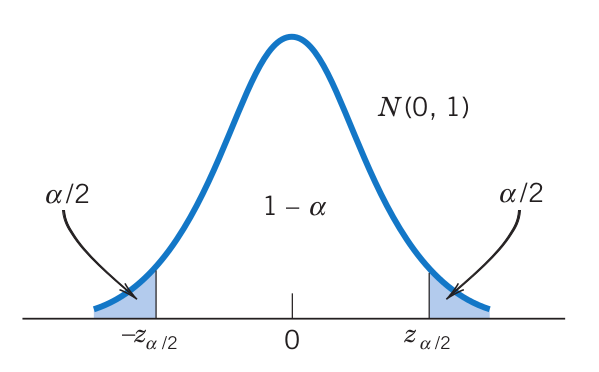
\includegraphics[scale=0.3]{8-2.png}
	\caption{The notation $z_{\alpha/2}$.}
\end{figure}
\begin{center}\begin{tabular}{c||ccc|ccc|ccc|ccc|ccc}
		\toprule[1.5pt]
		$1-\alpha$ && .80 &&& .85 &&& .90 &&& 0.95 &&& 0.99 &\\
		\hline
		$z_{\alpha/2}$ && 1.28 &&& 1.44 &&& 1.645 &&& 1.96 &&& 2.58 &\\
		\bottomrule[1.5pt]
	\end{tabular}
\end{center}

\begin{tcolorbox}[colback=white]\begin{center}
		\textcolor{blue}{\bf Point Estimation of the Mean}
	\end{center}
	\textcolor{blue}{Parameter:} Population mean $\mu$. \\
	\textcolor{blue}{\ \ \ \ \ \  \ Data:} $X_1,X_2,\cdots,X_n$ (a random sample of size $n$)\\
	\textcolor{blue}{\ Estimator:} $\overline{X}$ (sample mean) \\
	\[
	\SE(\overline{X})=\frac{\sigma}{\sqrt{n}}\qquad\text{Estimated}\ \SE(\overline{X}) = \frac{S}{\sqrt{n}}
	\] For large $n$, the $100(1-\alpha)\%$ error margin is $z_{\alpha/2}\sigma/\sqrt{n}$. (If $\sigma$ is unknown, use $S$ in place of $\sigma$.)
\end{tcolorbox} Note that $\dispsty S=\sqrt{\frac{\sum(X-\overline{X})}{n-1}}$.

\subsubsection*{* Determining the Sample Size}
Let \[
d =\ \text{Desired error margin}
\] and \[
1-\alpha =\ \text{Probability associated with error margin}.
\] Referring to the expression for a $100(1-\alpha)\%$ error margin, we then equate: \[
z_{\alpha/2}\frac{\sigma}{\sqrt{n}}=d.
\]
\begin{tcolorbox}[colback=white]
	To be $100(1-\alpha)\%$ sure that error of estimation $\abs{\overline{X}-\mu}$ does not exceed $d$, the \textbf{required sample size} is \[
	n=\left[\frac{z_{\alpha/2}\sigma}{d}\right]^2
	\]
\end{tcolorbox}

\subsection{Confidence Interval for a Population Mean}
Ideally, we would like to be able to collect a sample and then use it to calculate an interval that would definitely contain the true value of the parameter. This goal, however, is not achievable because of sample-to-sample variation. Instead, we insist that before sampling the proposed interval will contain the true
value with a specified high probability. This probability, called \textcolor{blue}{\bf the level of confidence}, is typically taken as .90, .95, or .99.\par
The normal table shows that the probability is .95 that a normal random variable will lie within 1.96 standard deviation from its mean. For $\overline{X}$, we have \[
P\left[\mu-1.96\frac{\sigma}{\sqrt{n}}<\overline{X}<\mu+1.96\frac{\sigma}{\sqrt{n}}\right] = .95
\iff P\left[\overline{X}-1.96\frac{\sigma}{\sqrt{n}}<\mu<\overline{X}+1.96\frac{\sigma}{\sqrt{n}}\right] = .95.
\]
\begin{figure}[h!]
	\centering
	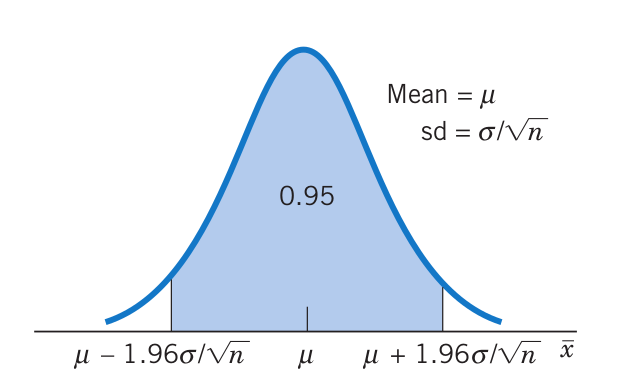
\includegraphics[scale=0.3]{8-3.png}
	\caption{Normal distribution of $\overline{X}$.}
\end{figure}\
\\
We say that the interval \[
\left(\overline{X}-1.96\frac{\sigma}{\sqrt{n}},\quad \overline{X}+1.96\frac{\sigma}{\sqrt{n}}\right)
\] or its realization $\left(\overline{x}-1.96\sigma/\sqrt{n},\ \overline{x}+1.96\sigma/\sqrt{n} \right)$ is a \textcolor{blue}{\bf 95\% confidence interval for $\boldsymbol{\mu}$} when the population is normal and $\sigma$ known. \par
We need not always tie our discussion of confidence intervals to the choice of a 95\% level of confidence. An investigator may wish to specify a different high probability. We denote this probability by $1-\alpha$ and speak of a $100(1-\alpha)\%$ \textcolor{blue}{\bf confidence interval}.\par
In summary, when the population is normal and $\sigma$ is known, a $100(1-\alpha)\%$ confidence interval for $\mu$ is given by \[
\left(\overline{X}-z_{\alpha/2}\frac{\sigma}{\sqrt{n}},\quad\overline{X}+z_{\alpha/2}\frac{\sigma}{\sqrt{n}} \right).
\]
\\
\subsubsection*{* Large Sample Confidence Intervals for $\mu$}
The central limit theorem then tells us that $\overline{X}$ is nearly normal whatever the form of the
population. We find that the large sample confidence interval for $\mu$ has the form \begin{center}
	Estimate\ $\pm$\ ($z$ value)(Estimated standard error).
\end{center}

\begin{tcolorbox}[colback=white]\begin{center}
		\textcolor{blue}{\bf Large Sample Confidence Interval for $\mu$}
	\end{center}
	When $n$ is large, a $100(1-\alpha)\%$ confidence interval for $\mu$ is given by \[
	\left(\overline{X}-z_{\alpha/2}\frac{S}{\sqrt{n}},\quad\overline{X}+z_{\alpha/2}\frac{S}{\sqrt{n}} \right)
	\] where $S$ is the sample standard deviation.
\end{tcolorbox}

\subsubsection*{* Confidence Interval for a Parameter}
The concept of a confidence interval applies to any parameter, not just the mean.
\begin{tcolorbox}[colback=white]\begin{center}
		\textcolor{blue}{\bf Definition of a Confidence Interval for a Parameter}
	\end{center}
	An interval $(L, U)$ is a $100(1-\alpha)\%$ confidence interval for a parameter if \[
	P\left[L<\ \text{Parmeter}\ < U \right] = 1-\alpha
	\] and the endpoints $L$ and $U$ are computable from the sample.
\end{tcolorbox}

\subsection{Testing Hypotheses about a Population Mean}
The formulation of a hypotheses testing problem and then the steps for solving it require a number of definitions and concepts. We will introduce these key statistical concepts \begin{quote}
	\textcolor{blue}{\bf Null hypothesis} and the \textcolor{blue}{\bf alternative hypothesis} \\
	\textcolor{blue}{\bf Type I} and \textcolor{blue}{\bf Type II errors} \\
	\textcolor{blue}{\bf Level of significance} \\
	\textcolor{blue}{\bf Rejection region} \\
	\textcolor{blue}{\bf P-value}
\end{quote} in the context a specific problem to help integrate them with intuitive reasoning.

\subsubsection*{* Formulating the Hypothesis}
In the language of statistics, the claim or the research hypothesis that we wish to establish is called the \textcolor{blue}{\bf alternative hypothesis $H_1$}. The opposite statement, one that nullifies the research hypothesis, is called \textcolor{blue}{\bf the null hypothesis $H_0$}.
\\
\begin{tcolorbox}[colback=white]\begin{center}
		\textcolor{blue}{\bf Formulation of $\boldsymbol{H_0}$ and $\boldsymbol{H_1}$}
	\end{center} When our goal is to establish an assertion with substantive support obtain from the sample, the negation of the assertion is taken to be the null hypothesis $H_0$ and the assertion itself is taken to be the alternative hypothesis $H_1$.
\end{tcolorbox}\ \\
Our initial question, ``Is there strong evidence in support of the claim?'' now
translates to ``Is there strong evidence for rejecting $H_0$?'' \\
\\
A \textcolor{blue}{\bf decision rule}, or a \textcolor{blue}{\bf test of the null hypothesis}, specifies a course of action by stating what sample information is to be used and how it is to be used in
making a decision. Bear in mind that we are to make one of the following two
decisions:
\begin{tcolorbox}[colback=white]\begin{center}
		\textcolor{blue}{\bf Decisions}
	\end{center} Either \[
	\text{Reject $H_0$ and conclude that $H_1$ is substantiated}
\] or \[
\text{Retain $H_0$ and conclude that $H_1$ fails to be substantiated}
\]
\end{tcolorbox}

\subsubsection*{* Test Criterion and Rejection Region}
A reasonable decision rule should be of the form \begin{align*}
\text{Reject}\ H_0\ &\text{if}\ \overline{X}\leq c \\
\text{Retain}\ H_0\ &\text{if}\ \overline{X}> c
\end{align*} This decision rule is conveniently expressed as $R:\overline{X}\leq c$, where $R$ stands for the rejection of $H_0$. The set of outcomes $[\overline{X}\leq c ]$ is called \textcolor{blue}{\bf rejection region} or \textcolor{blue}{\bf critical region}, and the cut-off point $c$ is called the \textcolor{blue}{\bf critical value}.
\\
\begin{tcolorbox}[colback=white]
The random variable $\overline{X}$ whose value serves to determine the action is called the 
\textcolor{blue}{\bf test statistic}. \\ 
A \textcolor{blue}{\bf test of the null hypothesis} is a course of action specifying the set of values of a test statistic $\overline{X}$, for which $H_0$ is to be rejected. \\
This set is called the \textcolor{blue}{\bf rejection region} of the test.
\end{tcolorbox}

\subsubsection*{* Two Types of Error and their Probabilities}
\begin{table}[h!]\centering
	\begin{tabular}{c||c|c}
		\toprule[1.5pt]
		\multirow{2}{*}{Decision Based on Sample} & \multicolumn{2}{c}{Unknown True Situation}   \\ \cline{2-3} 
		 & $H_0$ True & $H_1$ True \\ \hline\hline
		\multirow{2}{*}{Reject $H_0$} & Wrong rejection of $H_0$ & \multirow{2}{*}{Correct decision} \\
		 & (Type I error) &           \\ \hline
		\multirow{2}{*}{Retain $H_0$} &  \multirow{2}{*}{Correct decision} & Wrong retention of $H_0$ \\
		&           & (Type II error) \\
		\bottomrule[1.5pt]
	\end{tabular}
\end{table}
\begin{tcolorbox}[colback=white]\begin{center}
		\textcolor{blue}{\bf Two Types of Error}
	\end{center}
	\textcolor{blue}{\bf Type I error}: Rejection of $H_0$ when $H_0$ is true \\
	\textcolor{blue}{\bf Type II error}: Non-rejection of $H_0$ when $H_1$ is true \begin{align*}
	\alpha &=\ \text{Probability of making a Type I error} \\
	\beta &=\ \text{Probability of making a Type II error} \\
	\end{align*}
\end{tcolorbox} Here, $\alpha$ also called the \textcolor{blue}{\bf level of significance}. \\
\\
We hold a at a predetermined low level such as .10, .05, or .01 when choosing a rejection region. We will not pursue the evaluation of $\beta$, but we do note that if the $\beta$ turns out to be uncomfortably large, the sample size must be increased.

\subsubsection*{* P-value: How Strong Is a Rejection of $H_0$?}

\begin{tcolorbox}[colback=white]
	The \textcolor{blue}{\bf $P$-value}(or \textcolor{blue}{\bf significance probability}) is the probability, calculated under $H_0$, that the test statistic takes a value equal to or more extreme than the value actually observed.
\end{tcolorbox}\
\\ The \textcolor{blue}{\bf $P$-value} serves as a measure of the strength of evidence against $H_0$. A \textcolor{blue}{\bf small $P$-value} means that the null hypothesis is strongly rejected or the result is \textcolor{blue}{\bf highly statistically significant}.

\begin{tcolorbox}[colback=white]\begin{center}
		\textcolor{blue}{\bf The Steps for Testing Hypotheses}
	\end{center} \begin{enumerate}
	\item Formulate the null hypothesis $H_0$ and the alternative hypothesis $H_1$.
	\item Test criterion: State the test statistic and the form of the rejection region.
	\item With a specified a, determine the rejection region.
	\item Calculate the test statistic from the data.
	\item Draw a conclusion: State whether or not $H_0$ is rejected at the specified a and interpret the conclusion in the context of the problem. Also, it is a good statistical practice to calculate the $P$-value and strengthen the conclusion.
\end{enumerate}
\end{tcolorbox}
\
\begin{tcolorbox}[colback=white]\begin{center}
	\textcolor{blue}{\bf Large Sample Test for $\boldsymbol{\mu}$}
\end{center} When the sample size is large, a \textcolor{blue}{\bf $Z$ test} concerning $\mu$ is based on the normal test statistic \[
Z=\frac{\overline{X}-\mu_0}{S/\sqrt{n}}
\] The rejection region is one- or two-sided depending on the alternative hypothesis. Specifically,
\[\begin{array}{ccc}
H_1: \mu>\mu_0 && R:Z\geq z_\alpha \\
H_1: \mu<\mu_0 &\text{requires}& R:Z\geq -z_\alpha \\
H_1: \mu\neq\mu_0 && R:\abs{Z}\geq z_{\alpha/2}
\end{array}\]
\end{tcolorbox}

\subsection{Inferences about a Population Mean}
When $n$ elements are randomly sampled from the population, the data will consist of the count $X$ of the number of sampled elements possessing the characteristic. Common sense suggests the sample proportion \[
\hat{p}=\frac{X}{n}
\] as an estimator of $p$. The hat notation reminds us that $\hat{p}$ is a statistic.\par
When $n$ is large, the binomial variable $X$ is well approximated by a normal with mean $np$ and standard deviation $\sqrt{npq}$. That is, \[
Z=\frac{X-np}{\sqrt{npq}}
\] is approximately standard normal. In summary, when $n$ is large, $X\sim B(n,p)\approx N(np,np(1-p))$. Specially, \[
Z=\frac{(X-np)/n}{(\sqrt{npq})/n}=\frac{\hat{p}-p}{\sqrt{pq/n}}\approx N(0,1).
\] It shows that $\hat{p}$ is approximately normally distributed with mean $p$ and standard deviation $\sqrt{pq/n}$.
\\
\begin{figure}[h!]
	\centering
	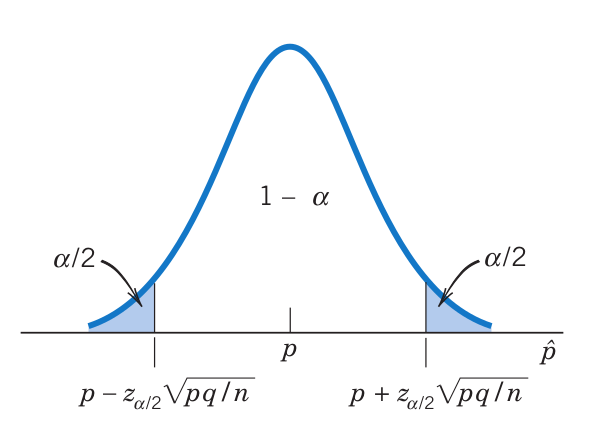
\includegraphics[scale=0.3]{8-5.png}
	\caption{Approximate normal distribution of $\hat{p}$.}
\end{figure}\

\newpage
\subsection*{* Point Estimation of $p$}
When the count $X$ has a binomial distribution, \[
E[X]=np\qquad \sd[X]=\sqrt{npq}.
\] Since $\hat{p}=X/n$, the properties of expectation give \[
E(\hat{p})=p\qquad\sd(\hat{p})=\sqrt{pq/n}.
\] The second result shows that \[
\SE(\hat{p})=\sqrt{\frac{pq}{n}}\qquad\text{and}\qquad\text{estimated}\ \SE(\hat{p})=\sqrt{\frac{\hat{p}\hat{q}}{n}}.
\] When $n$ is large, prior to sampling, the probability is approximately .954 that the error of estimation $\abs{\hat{p}-p}$ will be less than $2\times(\text{estimated}\ \SE)$. And when $n$ is large \[
P\left[-z_{\alpha/2}\leq\frac{\hat{p}-p}{\sqrt{\hat{p}(1-\hat{p})/n}}\leq z_{\alpha/2}\right]\approx1-\alpha.
\]

\begin{tcolorbox}[colback=white]\begin{center}
		\textcolor{blue}{\bf Point Estimation of a Population Proportion}
	\end{center} 
	\textbf{Parameter:} Population proportion $p$. \\
	\ \ \ \ \ \  \ \textbf{Data:} $X$ = Number having the characteristic in a random sample of size $n$\\
	\textbf{\ Estimator:} $\hat{p}=\dispsty\frac{X}{n}$ \\
	\[
	\SE(\hat{p})=\sqrt{\frac{pq}{n}}\qquad\text{and}\qquad\text{estimated}\ \SE(\hat{p})=\sqrt{\frac{\hat{p}\hat{q}}{n}}
	\] For large $n$, an approximate $100(1-\alpha)\%$ error margin is $z_{\alpha/2}\sqrt{\hat{p}\hat{q}/n}$.
\end{tcolorbox}

\subsection*{* Confidence Interval for $p$}

\begin{tcolorbox}[colback=white]\begin{center}
		\textcolor{blue}{\bf Large Sample Confidence Interval for $p$}
	\end{center} For large $n$, a $100(1-\alpha)\%$ confidence interval for $p$ is given by \[
	\left(\hat{p}-z_{\alpha/2}\sqrt{\frac{\hat{p}\hat{q}}{n}},\quad \hat{p}+z_{\alpha/2}\sqrt{\frac{\hat{p}\hat{q}}{n}}\right)
\] 
\end{tcolorbox}

\subsection*{* Determining the Sample Size}
The required sample size is obtained by equating \[
z_{\alpha/2}\sqrt{pq/n}=d,
\] where $d$ is the specified error margin. We then obtain \[
n=pq\left[\frac{z_{\alpha/2}}{d}\right]^2.
\] Without prior knowledge of $p, pq$ can be replaced by its maximum possible value $1/4$ and $n$ determined from the relation \[
n=\frac{1}{4}\left[\frac{z_{\alpha/2}}{d}\right]^2.
\]

\subsection*{* Large Sample Tests about $p$}
We consider testing $H_0:p=p_0$ versus $H_1:p\neq P_0$. With a large number of trials $n$, the sample proportion \[
\hat{p}=\frac{X}{n}
\] is approximately normally distributed. Under the null hypothesis, $p$ has the specified value $p_0$ and the distribution of $\hat{p}$ is approximately $N(p_0,\sqrt{p_0q_0/n})$. Consequently, the standardized statistic \[
Z=\frac{\hat{p}-p_0}{\sqrt{p_0q_0/n}}
\] has the $N(0,1)$ distribution. Note that \begin{enumerate}[(a)]
	\item $H_1:p>p_0\Rightarrow P=P(Z\geq z),\quad R:z\geq z_{\alpha}$
	\item $H_1:p<p_0\Rightarrow P=P(Z\leq z),\quad R:z\leq -z_{\alpha}$
	\item $H_1:p\neq p_0\Rightarrow P=P(\abs{Z}\geq \abs{z}),\quad R:\abs{z}\geq z_{\alpha/2}$
\end{enumerate}

\newpage
\section{Small Sample Inferences for Normal Populations}
\subsection{Unbiased Estimators}
\begin{tcolorbox}[colback=white]
	(\textbf{Unbiased Estimators for Expectation and Variance}) Suppose $X_1,X_2,\cdots,X_n$ is a random sample from a distribution with finite expectation $\mu$ and finite variance $\sigma^2$. Then \[
	\overline{X}_n=\frac{X_1+X_2+\cdots+X_n}{n}
	\] is an \textit{unbiased estimator for $\mu$}, i.e., $E[\overline{X}_n]=\mu$ and \[
	S_n^2=\frac{1}{n-1}\sum_{i=1}^n(X_i-\overline{X}_n)^2
	\] is an \textit{unbiased estimator for $\sigma^2$}, i.e., $E[S_n^2]=\sigma^2$.
\end{tcolorbox}\
\\
\textbf{Recall.} Let $X_1,X_2,\cdots,X_n$ are random sample. Then the followings hold:\begin{enumerate}[($i$)]
	\item $X_1,\cdots,X_n$ are mutually independent.
	\item Distribution of all $X_i$ = Population distribution.
\end{enumerate} This samples called \textbf{Independent and Identically Distributed (\textit{i.i.d.})} samples. Note that $\forall1\leq i\leq n$, \[
E[X_i]=\mu\quad\text{and}\quad \Var[X_i]=\sigma^2.
\]
\\
\textbf{Recall.} $E[\overline{X}_n]=\mu$. \begin{proof}\begin{align*}
	E[\overline{X}_n] &= \frac{1}{n}E[X_1+\cdots+X_n] \\
	&= \frac{1}{n}(E[X_1]+\cdots+E[X_n]) \\
	&= \frac{1}{n}(\mu+\cdots+\mu) = \mu.
	\end{align*}
\end{proof}\
\\ Now, we show that $E[S_n^2]=\sigma^2$. \begin{proof}
	Note that \[
		E[S_n^2]=\frac{1}{n-1}\sum_{i=1}^nE[(X_i-\overline{X}_n)^2].
	\] Since $E[X_n]=\mu$, we have $E[X_i-\overline{X}_n]=0$. Note that for any random variable $Y$ with $E[Y]=0$, we have \[
	\Var(Y)=E[Y^2]-(E[Y])^2=E[Y^2].
	\] Applying this to $Y=X_i-\overline{X}_n$, it follows that \[
	E[(X_i-\overline{X}_n)^2] = \Var(X_i-\overline{X}_n).
	\] Note that we can write \[
	X_i-\overline{X}_n=X_i-\frac{\sum X_i}{n} = \frac{nX_i-X_i-\sum_{j\neq i}X_j}{n}=\frac{n-1}{n}X_i-\frac{1}{n}\sum_{j\neq i}X_j.
	\] Then \begin{align*}
		\Var(X_i-\overline{X}_n) &= \Var\left(\frac{n-1}{n}X_i-\frac{1}{n}\sum_{j\neq i}X_j\right) \\
		&= \frac{(n-1)^2}{n^2}\Var(X_i)+\frac{1}{n^2}\sum_{j\neq i}\Var(X_j)\ \text{by independence of $X_j$'s} \\
		&= \left[\frac{(n-1)^2}{n^2}+\frac{n-1}{n^2}\right]\sigma^2=\frac{n-1}{n}\sigma^2.
	\end{align*} Hence, \begin{align*}
	E[S_n^2] &= \frac{1}{n-1}\sum_{i=1}^nE[(X_i-\overline{X}_n)^2]= \frac{1}{n-1}\sum_{i=1}^n\Var(X_i-\overline{X}_n) \\
	&= \frac{1}{n-1}\cdot n\cdot \frac{n-1}{n}\sigma^2=\sigma^2.
	\end{align*}
\end{proof}

\subsection{Student's $t$ Distribution}
\begin{tcolorbox}[colback=white]\begin{center}
		\textcolor{blue}{\bf Student's $\boldsymbol{t}$ Distribution}
	\end{center}
	If $X_1,\cdots,X_n$ is a random sample from a normal population $N(\mu,\sigma)$ and \[
	\overline{X}=\frac{1}{n}\sum X_i\qquad\text{and}\qquad S^2=\frac{\sum(X_i-\overline{X})^2}{n-1}
	\] then the distribution of \[
	T=\frac{\overline{X}-\mu}{S/\sqrt{n}}
	\] is called \textcolor{blue}{\bf Student's $\boldsymbol{t}$ distribution with $\boldsymbol{n-1}$ degrees of freedom}.
\end{tcolorbox}\begin{figure}[h!]
\centering
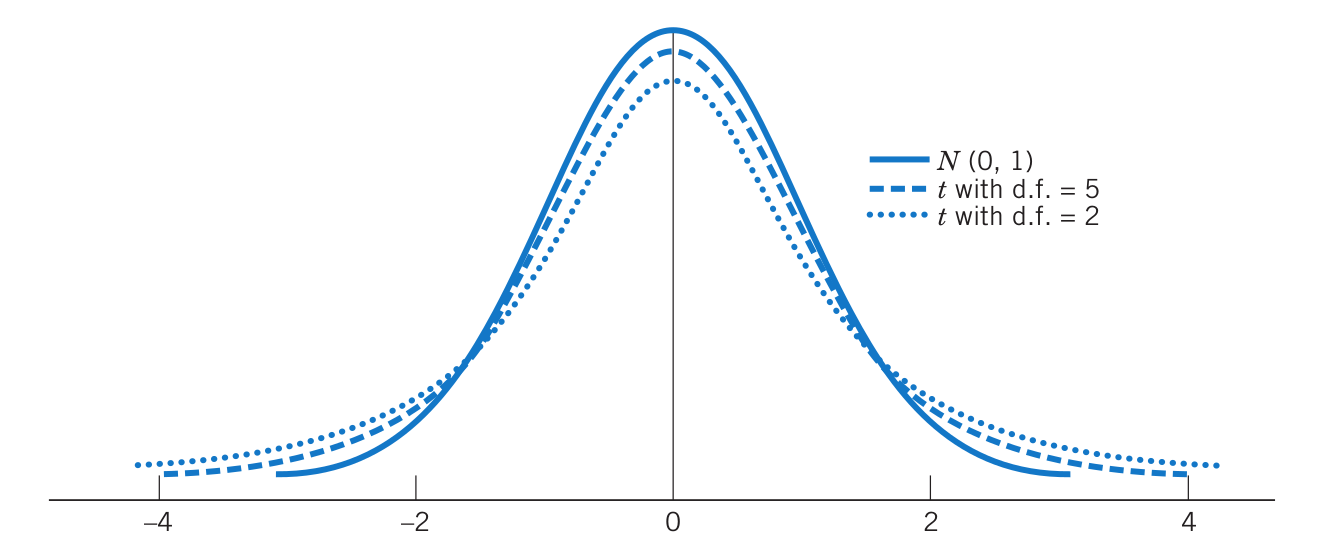
\includegraphics[scale=.28]{t_distribution.png}
\caption{Comparison of $N(0,1)$ and $t$ density curves.}
\end{figure}

\subsection{Inferences about $\mu$ - Small Sample Size}
\subsubsection{Confidence Interval for $\mu$}
The distribution of \[
T=\frac{\overline{X}-\mu}{S/\sqrt{n}}
\] provides the key for determining a \textcolor{blue}{\bf confidence interval for $\boldsymbol{\mu}$}, the mean of a normal population. \begin{figure}[h!]
	\centering
	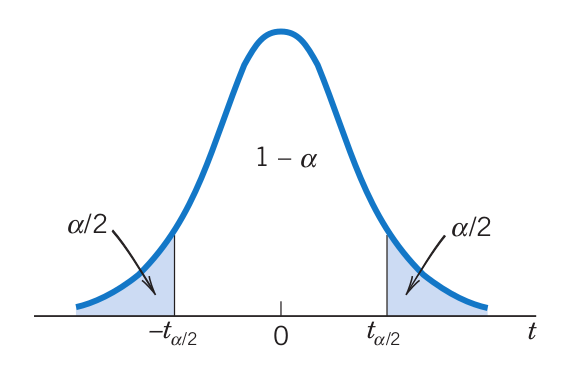
\includegraphics[scale=.3]{931.png}
	\caption{$t_{\alpha/2}$ and the probabilities.}
\end{figure}\
\\ Since $\dispsty\frac{\overline{X}-\mu}{S/\sqrt{n}}$ has the $t$ distribution with $\df = n-1$, we have \begin{align*}
1-\alpha &= P\left[-t_{\alpha/2}<\frac{\overline{X}-\mu}{S/\sqrt{n}}<t_{\alpha/2} \right] = P\left[-t_{\alpha/2}\frac{S}{\sqrt{n}}<\overline{X}-\mu<t_{\alpha/2}\frac{S}{\sqrt{n}} \right] \\
&= P\left[\overline{X}-t_{\alpha/2}\frac{S}{\sqrt{n}}<\mu<\overline{X}+t_{\alpha/2}\frac{S}{\sqrt{n}} \right].
\end{align*}
\begin{tcolorbox}[colback=white]\begin{center}
		\textcolor{blue}{\bf A $\boldsymbol{100(1-\alpha)\%}$ Confidence Interval for a Normal Population Mean}
	\end{center}\[
\left(\overline{X}-t_{\alpha/2}\frac{S}{\sqrt{n}},\quad \overline{X}+t_{\alpha/2}\frac{S}{\sqrt{n}}\right)
\] where $t_{\alpha/2}$ is the upper $\alpha/2$ point of the $t$ distribution with $\df=n-1$.
\end{tcolorbox}

\subsubsection{Hypothesis Tests for $\mu$}
\begin{tcolorbox}[colback=white]\begin{center}
		\textcolor{blue}{\bf Hypotheses Tests for $\boldsymbol{\mu}$ - Small Samples}
	\end{center}
	To test $H_0:\mu=\mu_0$ concerning the mean of a \textbf{normal population}, the test statistic is \[
	T=\frac{\overline{X}-\mu_0}{S/\sqrt{n}}
	\] which has Student's $t$ distribution with $n-1$ degrees of freedom: \begin{align*}
	H_1:\mu>\mu_0\qquad & R:T\geq t_\alpha \\
	H_1:\mu<\mu_0\qquad & R:T\leq -t_\alpha \\
	H_1:\mu\neq\mu_0\qquad & R:\abs{T}\geq t_{\alpha/2}
	\end{align*} The test is called a \textbf{Student's $\boldsymbol{t}$ test} or simply a \textbf{$\boldsymbol{t}$ test}.
\end{tcolorbox}

\subsection{Relationship between Tests and Confidence Intervals}

A $100(1-\alpha)\%$ confidence interval for $\mu$ is $\dispsty
\left(\overline{X}-t_{\alpha/2}\frac{S}{\sqrt{n}},\ \overline{X}+t_{\alpha/2}\frac{S}{\sqrt{n}}\right).
$ On the other hand, the rejection region of a level $\alpha$ test for $H_0:\mu=\mu_0$ versus the two-sided alternative $H_1:\mu\neq\mu_0$ is \[
R:\abs{\frac{\overline{X}-\mu_0}{S/\sqrt{n}}}\geq t_{\alpha/2}.
\] Reversing the inequality in $R$, we obtain Acceptance region: $\dispsty
-t_{\alpha/2}<\frac{\overline{X}-\mu_0}{S/\sqrt{n}}<t_{\alpha/2}
$ which can also be written as \[
\overline{X}-t_{\alpha/2}\frac{S}{\sqrt{n}}<\mu_0<\overline{X}+t_{\alpha/2}\frac{S}{\sqrt{n}}.
\]
\subsection{Inferences about the Standard Deviation $\sigma$ (The $\chi^2$ Distribution)}

\begin{tcolorbox}[colback=white]\begin{center}
		\textcolor{blue}{\bf $\boldsymbol{\chi^2}$ Distribution}
	\end{center} Let $X_1,\cdots,X_n$ be a random sample from a normal population $N(\mu,\sigma)$. Then the distribution of \[
\chi^2=\frac{\sum_{i=1}^n(X_i-\overline{X})^2}{\sigma^2}=\frac{(n-1)S^2}{\sigma^2}
\] is called the \textcolor{blue}{\bf $\boldsymbol{\chi^2}$ distribution with $\boldsymbol{n-1}$ degrees of freedom}.
\end{tcolorbox}\begin{figure}[h!]
\centering
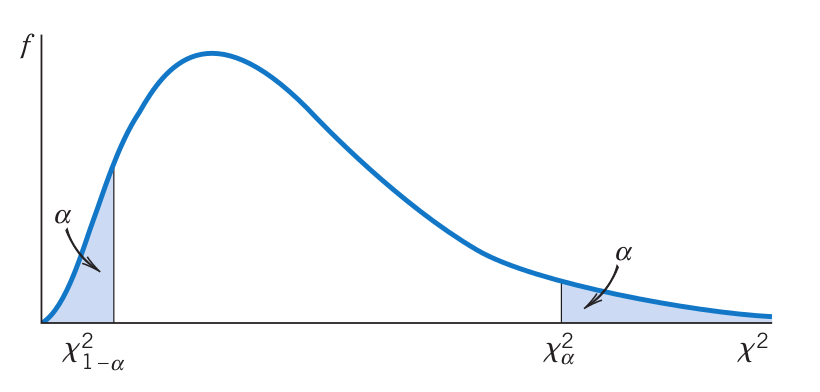
\includegraphics[scale=.3]{chi_square.png}
\caption{Probability density curve of a $\chi^2$ distribution.}
\end{figure}\
\\
The $\chi^2$ is the basic distribution for constructing intervals for $\sigma^2$ or $\sigma$. We outline the steps in terms of a 95\% confidence interval for $\sigma^2$. Dividing the probability $\alpha = .05$ equally between th two tails of the $\chi^2$ distribution, \[
P\left[\chi_{.975}^2<\frac{(n-1)S^2}{\sigma^2}<\chi_{.025}^2\right] = .95
\] where the percentage points are read from the $\chi^2$ table at $\df=n-1$. Also we have \[
P\left[\frac{(n-1)S^2}{\chi_{.025}^2}<\sigma^2<\frac{(n-1)S^2}{\chi_{.975}^2}\right] = .95.
\] Therefore, for a confidence level .95, the interval for $\sigma$ becomes \[
\left(S\sqrt{\frac{n-1}{\chi_{.025}^2}},\ S\sqrt{\frac{n-1}{\chi_{.975}^2}}\right).
\]

\subsection{Robustness of Inference Procedures}
The small sample methods for both confidence interval estimation and hypothesis testing presuppose that the sample is obtained from a normal population. Users of these methods would naturally ask: \begin{enumerate}
	\item What method can be used to determine if the population distribution is nearly normal?
	\item What can go wrong if the population distribution is non-normal?
	\item What procedures should be used if it is non-normal?
	\item If the observations are not independent, is this serious?
\end{enumerate}\
\par
1. To answer the first question, we could construct the dot diagram or normal-scores plot. \\\par
2. Fortunately, the effects on inferences about $\mu$ using the $t$ statistic are not too serious if the sample size is at least moderately large (say, 15). In larger samples, such disturbances tend to disappear due to the central limit theorem. We express this fact by saying that \textbf{inferences about $\boldsymbol{\mu}$ using the $\boldsymbol{t}$ statistic are reasonably} \textcolor{blue}{\bf ``robust''}.\\\par
3.\\\par
4.
\\
\\
%\begin{tcolorbox}[colback=white]\begin{center}
%	\textcolor{blue}{\bf Decisions}
%\end{center} 
%
%\end{tcolorbox}\begin{tcolorbox}[colback=white]\begin{center}
%	\textcolor{blue}{\bf Decisions}
%\end{center} 
%
%\end{tcolorbox}
%\begin{tcolorbox}[colback=white]
%	
%\end{tcolorbox}
%
%
%\begin{tcolorbox}[colback=white]
%	
%\end{tcolorbox}
%\begin{tcolorbox}[colback=white]
%	
%\end{tcolorbox}

\end{document}